% ============================================================
%  rapport_de_stage.tex - Rapport de stage CN-ITIE Senegal
%  Stage au service « Gestion des donnees » du Comite national ITIE
%  Sié Rachid TRAORÉ - ISE3, ENSAE Pierre Ndiaye (Dakar)
%  Compilation : xelatex (2 passes) - style herite de main.tex (ENSAE)
% ============================================================

\documentclass[12pt, a4paper]{article}

% ── Encodage & langue ────────────────────────────────────────
\usepackage[french]{babel}
\usepackage{csquotes}

% ── Mise en page ────────────────────────────────────────────
\usepackage[
  top=2.5cm, bottom=2.5cm,
  left=3cm, right=2.5cm,
  headheight=28pt
]{geometry}
\usepackage{setspace}
\onehalfspacing
\raggedbottom
\usepackage[indent=0pt, skip=8pt]{parskip}

% ── Police (Times New Roman si disponible, sinon Liberation Serif) ──
\usepackage{fontspec}
\IfFontExistsTF{Times New Roman}
  {\setmainfont{Times New Roman}}
  {\setmainfont{Liberation Serif}}
\usepackage{microtype}

% ── En-têtes et pieds de page ───────────────────────────────
\usepackage{fancyhdr}
\pagestyle{fancy}
\fancyhf{}
\renewcommand{\headrulewidth}{0pt}
\renewcommand{\footrulewidth}{0.4pt}
\fancyfoot[L]{\scriptsize Sié Rachid TRAORÉ, ISE3 (ENSAE-DAKAR)}
\fancyfoot[C]{\scriptsize\textbf{\{\,\thepage\,\}}}
\fancyfoot[R]{\scriptsize Rapport de stage CN-ITIE, 2026}

\fancypagestyle{plain}{%
  \fancyhf{}
  \renewcommand{\headrulewidth}{0pt}
  \renewcommand{\footrulewidth}{0.4pt}
  \fancyfoot[L]{\scriptsize Sié Rachid TRAORÉ, ISE3 (ENSAE-DAKAR)}
  \fancyfoot[C]{\scriptsize\textbf{\{\,\thepage\,\}}}
  \fancyfoot[R]{\scriptsize Rapport de stage CN-ITIE, 2026}
}

% ── Couleurs ENSAE ───────────────────────────────────────────
\usepackage[table]{xcolor}
\definecolor{ensaeblue}{RGB}{25,25,112}
\definecolor{ensaecyan}{RGB}{0,174,239}
\definecolor{ensaeorange}{RGB}{224,123,57}
\definecolor{tableline}{RGB}{180,180,180}
\definecolor{ensaerow}{RGB}{252,232,215}

% ── Style « tableur » (grille + en-tête orange + zébrage) ────
\arrayrulecolor{tableline}
\newcommand{\entete}{\rowcolor{ensaeorange}}
\newcommand{\zebre}{\rowcolors{2}{white}{ensaerow}}
\newcommand{\nozebre}{\rowcolors{1}{}{}}
\newcommand{\sousentete}{\rowcolor{ensaerow}}

% ── Titres de section - bandeau ENSAE ────────────────────────
\usepackage{titlesec}
\titlespacing*{\section}{0pt}{0pt}{4pt}
\titlespacing*{\subsection}{0pt}{8pt}{4pt}
\titlespacing*{\subsubsection}{0pt}{6pt}{3pt}

\newif\ifensaeenchaine
\ensaeenchainefalse

\setlength{\fboxsep}{6pt}
\newcommand{\ensaetetesection}[2]{%
  \par\begingroup\setlength{\parskip}{0pt}%
  \ifensaeenchaine
    \vspace{1.8cm}\global\ensaeenchainefalse
  \else
    \vspace*{-1.5cm}%
  \fi
  {\centering
   \parbox{0.78\textwidth}{\centering\color{ensaeblue}\Large\bfseries #1}\par}
  \vspace{0.12cm}
  \noindent
  \begin{tikzpicture}
    \ifx\relax#2\relax
      \fill[ensaeblue, rounded corners=3pt] (0,-3pt) rectangle (\textwidth,3pt);
    \else
      \fill[ensaeblue, rounded corners=3pt]
        (0,-3pt) rectangle (0.925\textwidth,3pt);
      \node[circle, fill=ensaeblue, text=white, minimum size=1.8cm,
            inner sep=0pt, overlay,
            font=\fontsize{36}{36}\selectfont] (pastille)
        at ([yshift=0.9cm]0.925\textwidth,-3pt) {#2};
    \fi
  \end{tikzpicture}\par
  \endgroup
  \vspace{0.45cm}
}
\newcommand{\ensaebandeaunum}[1]{\ensaetetesection{#1}{\thesection}}
\newcommand{\ensaebandeaunn}[1]{\ensaetetesection{#1}{}}

\titleformat{\section}[block]{\normalfont}{}{0pt}{\ensaebandeaunum}
\titleformat{name=\section,numberless}[block]{\normalfont}{}{0pt}{\ensaebandeaunn}

\titleformat{\subsection}
  {\normalfont\normalsize\bfseries\color{ensaeblue}}
  {\thesubsection.}{0.5em}{}

\titleformat{\subsubsection}
  {\normalfont\normalsize\bfseries\color{ensaeblue}}
  {\thesubsubsection.}{0.5em}{}

% ── Bordure de page ENSAE (double filet cyan) ────────────────
\usepackage{tikz}
\usetikzlibrary{positioning,calc}
\usepackage{eso-pic}
\newlength\ensaecoin
\setlength\ensaecoin{10pt}
\newcommand*\ensaecoinorange[1]{%
  \begin{scope}
    \clip #1;
    \fill[ensaeorange, even odd rule, rounded corners=9pt]
      (SW) rectangle (NE)
      [rounded corners=6pt] (sw) rectangle (ne);
  \end{scope}%
}
\newcommand{\ensaecadrepage}{%
  \AtPageLowerLeft{%
    \begin{tikzpicture}[overlay, line cap=round, line join=round]
      \coordinate (SW) at (15pt,15pt);
      \coordinate (NE) at ($(\paperwidth,\paperheight)-(15pt,15pt)$);
      \coordinate (sw) at (20pt,20pt);
      \coordinate (ne) at ($(\paperwidth,\paperheight)-(20pt,20pt)$);
      \coordinate (SE) at (NE|-SW);
      \coordinate (NW) at (SW|-NE);
      \ensaecoinorange{($(SW)+(-3pt,-3pt)$) rectangle ($(SW)+(\ensaecoin,\ensaecoin)$)}
      \ensaecoinorange{($(SE)+(3pt,-3pt)$)  rectangle ($(SE)+(-\ensaecoin,\ensaecoin)$)}
      \ensaecoinorange{($(NW)+(-3pt,3pt)$)  rectangle ($(NW)+(\ensaecoin,-\ensaecoin)$)}
      \ensaecoinorange{($(NE)+(3pt,3pt)$)   rectangle ($(NE)+(-\ensaecoin,-\ensaecoin)$)}
      \draw[ensaeblue, line width=1.7pt, rounded corners=9pt] (SW) rectangle (NE);
      \draw[ensaecyan, line width=0.6pt, rounded corners=6pt] (sw) rectangle (ne);
    \end{tikzpicture}%
  }%
}

% ── Figures & tableaux ──────────────────────────────────────
\usepackage{graphicx}
\usepackage{float}
\usepackage{booktabs}
\usepackage{longtable}
\usepackage{array}
\usepackage{makecell}
\usepackage{multirow}
\usepackage{caption}
\captionsetup{font=small, labelfont=bf, labelsep=period}
\usepackage{tabularx}

% ── Liens & PDF ─────────────────────────────────────────────
\usepackage[
  colorlinks=true,
  linkcolor=ensaeblue,
  citecolor=ensaeorange,
  urlcolor=ensaeblue,
  linktoc=all,
  bookmarks=true,
  pdftitle={Rapport de stage - CN-ITIE Senegal - Service Gestion des donnees},
  pdfauthor={Sie Rachid TRAORE},
  pdfsubject={Rapport de stage - CN-ITIE / ENSAE Dakar}
]{hyperref}

% ── Listes ──────────────────────────────────────────────────
\AtBeginDocument{\renewcommand{\labelitemi}{\textbullet}}
\usepackage{enumitem}
\setlist[itemize]{noitemsep, topsep=4pt, label=\textbullet}
\setlist[itemize,2]{label=$\circ$}
\setlist[enumerate]{noitemsep, topsep=4pt}

% ── Saut de page avant chaque \section ─────────────────────
\usepackage{etoolbox}
\pretocmd{\section}{\clearpage}{}{}

\setcounter{secnumdepth}{3}
\setcounter{tocdepth}{2}

% ============================================================
\begin{document}

% ── Page de garde ────────────────────────────────────────────
\AddToShipoutPictureBG*{\ensaecadrepage}
\begin{titlepage}
  \begin{center}
    {\small\bfseries RÉPUBLIQUE DU SÉNÉGAL}\\[0.1cm]
    {\scriptsize Un Peuple - Un But - Une Foi}\\[0.4cm]
    \begin{minipage}[t]{0.45\textwidth}
      \centering
      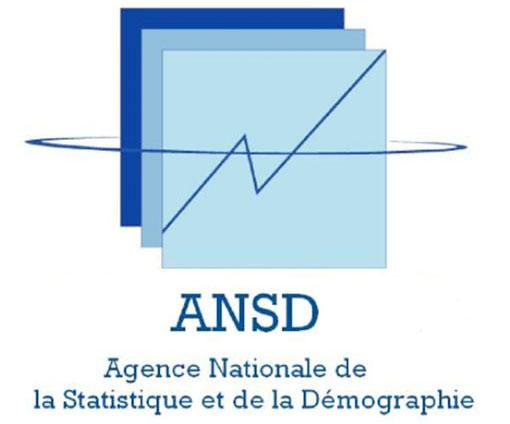
\includegraphics[height=1.9cm]{ANSD.jpg}\\[0.15cm]
      
\includegraphics[height=2.0cm]{ensae.png}\\[0.05cm]
      {\scriptsize\bfseries École Nationale de la Statistique\\ et de l'Analyse Économique Pierre Ndiaye}
    \end{minipage}\hfill
    \begin{minipage}[t]{0.45\textwidth}
      \centering
      {\scriptsize\bfseries Présidence de la République}\\[0.2cm]
      
\includegraphics[height=2.1cm]{Itie.png}\\[0.15cm]
      {\scriptsize\bfseries Comité national ITIE Sénégal}
    \end{minipage}\\[1.2cm]

    \begin{tikzpicture}
      % Bandeau principal : fond bleu ENSAE, coins arrondis, filet cyan
      % interieur et pastilles orange aux extremites (rappel du cadre de page).
      \node[fill=ensaeblue, rounded corners=10pt, inner ysep=15pt,
            text width=0.88\textwidth, align=center] (titre) at (0,0)
        {\color{white}\Huge\bfseries\scshape Rapport de stage};
      \draw[ensaecyan, line width=0.6pt, rounded corners=7pt]
        ([xshift=4pt,yshift=-4pt]titre.north west)
          rectangle ([xshift=-4pt,yshift=4pt]titre.south east);
      \fill[ensaeorange] (titre.west) circle (3.5pt);
      \fill[ensaeorange] (titre.east) circle (3.5pt);
      % Cartouche du sous-titre : fond orange tres clair, lisere bleu
      \node[below=0.45cm of titre, fill=ensaerow, draw=ensaeblue,
            line width=0.8pt, rounded corners=8pt, inner ysep=11pt,
            text width=0.82\textwidth, align=center] (soustitre)
        {\color{ensaeblue}\large Appui à la gestion des données du secteur
         extractif\\[3pt]
         \color{ensaeblue}\large Fiabilisation du Registre des Bénéficiaires
         Effectifs et analyse du sous-secteur de l'EMAPE par la statistique
         miroir};
      % Trait de liaison entre bandeau et cartouche
      \draw[ensaeorange, line width=1.6pt]
        ([yshift=1pt]titre.south) -- ([yshift=-1pt]soustitre.north);
    \end{tikzpicture}\\[0.7cm]

    {\normalsize Stage effectué au sein du \textbf{Comité national de l'Initiative pour la
    Transparence dans les Industries Extractives (CN-ITIE)}, Service « Gestion des données »}\\[0.3cm]
    {\normalsize\itshape Ngor-Almadies, Dakar, du 04 mai au 31 juillet 2026}\\[1.1cm]

    \begin{tabular}{p{0.46\textwidth}p{0.46\textwidth}}
      \textbf{Présenté par :} & \textbf{Encadreur :}\\[0.15cm]
      Sié Rachid TRAORÉ & M. Fallou DIONE\\
      Élève Ingénieur Statisticien & \emph{Gestionnaire de données, CN-ITIE}\\[0.15cm]
      Économiste (ISE3) & \textbf{Supervision :}\\[0.15cm]
      ENSAE Pierre Ndiaye, Dakar & M. Thaddée Adiouma SECK\\
      & \emph{Secrétaire Permanent du CN-ITIE}\\
    \end{tabular}\\[1.2cm]

    {\color{ensaeblue}\bfseries Année académique 2025-2026}
  \end{center}
\end{titlepage}

% ── Pages liminaires ─────────────────────────────────────────
\pagestyle{plain}
\pagenumbering{roman}
\setcounter{page}{1}

\section*{Remerciements}
\addcontentsline{toc}{section}{Remerciements}

Je tiens à exprimer ma profonde gratitude à l'ensemble du personnel du Comité
national de l'Initiative pour la Transparence dans les Industries Extractives
(CN-ITIE) du Sénégal pour la qualité de l'accueil qui m'a été réservé durant ces
trois mois de stage.

Mes remerciements s'adressent en premier lieu à Monsieur Thaddée Adiouma
SECK, Secrétaire Permanent du CN-ITIE, pour m'avoir ouvert les portes de
l'institution et pour la confiance accordée dans le traitement de données
sensibles du secteur extractif.

Je remercie tout particulièrement Monsieur Fallou DIONE, Gestionnaire de
données et encadreur du stage, pour son suivi hebdomadaire rigoureux, ses
orientations méthodologiques et la validation attentive de chacun des livrables.

Ma reconnaissance va également à l'ensemble de l'équipe du Secrétariat Technique
du CN-ITIE pour leur disponibilité, ainsi qu'à mon binôme de stage,
Rasmané BAMOGO, avec qui les travaux communs sur le Registre des
Bénéficiaires Effectifs ont été menés dans un esprit de collaboration exemplaire.

Enfin, je remercie l'École Nationale de la Statistique et de l'Analyse Économique
(ENSAE) Pierre Ndiaye, dont le consortium établi avec le CN-ITIE a rendu possible
cette immersion professionnelle.

\clearpage

\section*{Avant-propos}
\addcontentsline{toc}{section}{Avant-propos}

Le présent rapport est établi en application de l'article 8 du contrat de stage
signé entre le CN-ITIE et le stagiaire, qui dispose qu'à la fin du stage un
rapport écrit est soumis à la structure d'accueil. Il rend compte du déroulement
du stage effectué du 04 mai au 31 juillet 2026 au service « Gestion des données »
du CN-ITIE, des travaux réalisés au regard du cahier des charges, des résultats
obtenus, ainsi que des compétences acquises.

Conformément aux articles 4 et 7 du contrat de stage, les données individuelles
traitées durant le stage demeurent confidentielles. Le présent rapport ne
restitue que des résultats agrégés et des éléments méthodologiques, à
l'exclusion de toute donnée nominative non publique.

Un état de suivi détaillé des travaux, précisant pour chaque tâche si elle est
réalisée, partiellement réalisée ou non réalisée, et assorti de commentaires,
figure en annexe~\ref{annexe:suivi}.

\clearpage

\section*{Sigles et abréviations}
\addcontentsline{toc}{section}{Sigles et abréviations}

\begin{tabular}{p{3cm}p{11.5cm}}
  \textbf{AMA} & Autorisation minière artisanale\\
  \textbf{AMSM} & Autorisation minière semi-mécanisée\\
  \textbf{ANSD} & Agence Nationale de la Statistique et de la Démographie\\
  \textbf{BCEAO} & Banque Centrale des États de l'Afrique de l'Ouest\\
  \textbf{BE} & Bénéficiaire effectif\\
  \textbf{CN-ITIE} & Comité national de l'Initiative pour la Transparence dans les Industries Extractives\\
  \textbf{DCSOM} & Direction du Contrôle et de la Surveillance des Opérations Minières\\
  \textbf{DGI} & Direction Générale des Impôts\\
  \textbf{DGMG} & Direction Générale des Mines et de la Géologie\\
  \textbf{DREPM} & Direction régionale de l'Énergie, du Pétrole et des Mines\\
  \textbf{EMAPE} & Exploitation Minière Artisanale et à Petite Échelle\\
  \textbf{ENSAE} & École Nationale de la Statistique et de l'Analyse Économique\\
  \textbf{FARI} & Fiscal Analysis of Resource Industries (modèle FMI)\\
  \textbf{GAFI} & Groupe d'Action Financière\\
  \textbf{GMP} & Groupe Multipartite\\
  \textbf{ISE} & Ingénieur Statisticien Économiste\\
  \textbf{ISIN} & International Securities Identification Number\\
  \textbf{ITIE} & Initiative pour la Transparence dans les Industries Extractives\\
  \textbf{MEPM} & Ministère de l'Énergie, du Pétrole et des Mines\\
  \textbf{OE} & (Programme) Propriété effective / \emph{Ownership Engagement}\\
  \textbf{PPE} & Personne Politiquement Exposée\\
  \textbf{RBE} & Registre des Bénéficiaires Effectifs\\
  \textbf{RCCM} & Registre du Commerce et du Crédit Mobilier\\
  \textbf{SH} & Système Harmonisé (nomenclature douanière)\\
  \textbf{UE} & Union Européenne\\
\end{tabular}

\clearpage

% ── Sommaire ─────────────────────────────────────────────────
\begin{singlespace}
\tableofcontents
\end{singlespace}
\clearpage

% ── Corps du rapport ─────────────────────────────────────────
\pagestyle{fancy}
\pagenumbering{arabic}
\setcounter{page}{1}

\section{Introduction}

Dans le cadre du consortium établi entre l'École Nationale de la Statistique et
de l'Analyse Économique (ENSAE) Pierre Ndiaye et le Comité national de
l'Initiative pour la Transparence dans les Industries Extractives (CN-ITIE) du
Sénégal, deux élèves en dernière année du cycle Ingénieur Statisticien
Économiste ont été accueillis en stage pour une durée de trois mois.
J'ai ainsi effectué, du 04 mai au 31 juillet 2026, un stage au service
« Gestion des données » du CN-ITIE, sous la supervision du Secrétaire Permanent,
Monsieur Thaddée Adiouma SECK, et l'encadrement technique du Gestionnaire de
données, Monsieur Fallou DIONE.

Le stage s'inscrit dans un contexte de renforcement structurel des capacités
d'analyse, de contrôle et de gouvernance du secteur extractif sénégalais. Le
cahier des charges qui l'encadre lui assigne deux objectifs principaux :

\begin{itemize}
  \item fiabiliser et enrichir le Registre des Bénéficiaires Effectifs
  (RBE) des sociétés extractives, en assurant une conformité renforcée avec
  l'exigence 2.5 de la Norme ITIE 2023 ;
  \item produire une base analytique robuste sur les Exploitations
  Minières Artisanales et à Petite Échelle (EMAPE), incluant l'estimation des
  volumes de production par la méthode des statistiques miroir et la
  cartographie des circuits de commercialisation et des acteurs de la chaîne de
  valeur.
\end{itemize}

Le dispositif de stage reposait sur un lot commun obligatoire consacré au
registre des bénéficiaires effectifs, mené conjointement avec mon binôme
M. Rasmané BAMOGO durant les six premières semaines, puis sur un lot
thématique individuel consacré à l'exploitation minière artisanale, mené en
parallèle à compter de la troisième semaine. Le stage était explicitement « orienté
résultats ». Les livrables constituaient des obligations contractuelles, tout
choix méthodologique devait être justifié, les scripts documentés et
reproductibles, et les sources systématiquement référencées.

Le présent rapport s'articule en quatre parties. La première présente la
structure d'accueil et le cadre du stage. La deuxième détaille les travaux
menés sur le Registre des Bénéficiaires Effectifs, à savoir l'audit de qualité
des données 2021-2025 et le développement de la plateforme de consultation
\emph{OpenRBE}. La troisième expose les travaux sur le sous-secteur de l'EMAPE
et l'application de la méthode des statistiques miroir aux flux d'or
2020-2024. La quatrième restitue les travaux transverses d'appui au service,
puis dresse le bilan du stage (résultats, difficultés, compétences acquises et
recommandations).

\section{Présentation de la structure d'accueil et cadre du stage}

\subsection{Le Comité national ITIE du Sénégal}

L'Initiative pour la Transparence dans les Industries Extractives (ITIE) est la
norme mondiale de référence pour la gouvernance transparente et redevable des
ressources pétrolières, gazières et minières. Le Sénégal, pays de mise en
œuvre, s'appuie sur un Comité national créé par le décret
n°~2013-881 du 20 juin 2013, abrogé et remplacé par le décret n°~2021-1145 du
7~septembre 2021 fixant les règles de son organisation et de son
fonctionnement. Son siège est situé à Ngor-Almadies, sur le site dit « IPRES », à Dakar.

Le CN-ITIE est une structure tripartite regroupant des représentants du
Gouvernement, des entreprises extractives et de la société civile. Il est
chargé de superviser la mise en œuvre de la Norme ITIE au Sénégal, notamment à
travers :

\begin{itemize}
  \item la collecte et la réconciliation des données sur les revenus du secteur
  extractif, c'est-à-dire les flux financiers entre les entreprises et l'État ;
  \item la divulgation des informations relatives à la propriété effective des
  entreprises extractives ;
  \item la production des rapports annuels ITIE et le renforcement de la
  transparence dans la gestion des ressources minières, pétrolières et
  gazières.
\end{itemize}

Ses activités quotidiennes sont assurées par un Secrétariat Technique placé
sous l'autorité du Groupe Multipartite. Le service « Gestion des
données », au sein duquel le stage s'est déroulé, est responsable de la
collecte, de la structuration, du contrôle qualité et de la valorisation des
données du périmètre ITIE.

\subsection{Cadre contractuel et organisation du stage}

Le stage a été formalisé par un contrat signé avec le CN-ITIE, complété par un
cahier des charges détaillé. Les principaux éléments du dispositif sont
récapitulés ci-dessous.

\begin{table}[H]
\centering
\caption{Fiche synthétique du stage}
\zebre
\begin{tabular}{p{4.5cm}p{9.5cm}}
  \entete
  \textcolor{white}{\textbf{Élément}} & \textcolor{white}{\textbf{Description}}\\
  Structure d'accueil & CN-ITIE Sénégal, service « Gestion des données »\\
  Période & 04 mai - 31 juillet 2026 (3 mois, 12 semaines)\\
  Stagiaire & Sié Rachid TRAORÉ, élève ISE3 (ENSAE Pierre Ndiaye)\\
  Binôme & Rasmané BAMOGO (lot commun RBE)\\
  Supervision & M. Thaddée Adiouma SECK, Secrétaire Permanent\\
  Encadreur & M. Fallou DIONE, Gestionnaire de données\\
  Suivi & Points hebdomadaires (30 min) sur compte rendu d'avancement ; revue formelle de mi-parcours ; présentation finale devant l'équipe\\
  Obligations & Confidentialité des données, scripts reproductibles, sources référencées, validation des livrables avant diffusion\\
\end{tabular}
\nozebre
\end{table}

Le calendrier prévisionnel du cahier des charges structurait le stage en quatre
phases, le cadrage et la collecte en semaines 1 et 2, la structuration des
bases en semaines 3 à 6, l'analyse et la modélisation en semaines 7 à 9, puis
les livrables finaux en semaines 10 à 12. Les travaux qui
m'étaient assignés couvraient le lot commun RBE et le lot thématique EMAPE ;
la modélisation économétrique des coûts de production relevait du lot de mon
binôme.

\section{Travaux sur le Registre des Bénéficiaires Effectifs}

L'exigence 2.5 de la Norme ITIE 2023 impose la divulgation de l'identité des
bénéficiaires effectifs de toutes les sociétés extractives détentrices de
licences actives. Au Sénégal, ce cadre est décliné par le décret n°~2020-791 du
19 mars 2020 et ses modificatifs, dont le récent décret n°~2025-1354 relatif au
registre des bénéficiaires effectifs. Le diagnostic conduit en 2024 dans le cadre du programme de divulgation de la
propriété effective avait révélé des lacunes importantes :
sociétés sans déclaration, qualité insuffisante des données, absence
d'identifiants communs entre registres administratifs. Les travaux RBE du stage
visaient à objectiver puis résorber ces lacunes.

\subsection{Revue documentaire et collecte}

La phase de cadrage a consisté à constituer et exploiter un corpus
réglementaire et méthodologique comprenant la Norme ITIE 2023 en son exigence 2.5, le décret
n°~2020-791 et ses modificatifs, le décret n°~2025-1354, l'arrêté ministériel
n°~1598 relatif au formulaire de déclaration des bénéficiaires effectifs et les
codes minier et pétrolier, ainsi que le diagnostic précité de 2024 et le projet d'étude
« Bénéficiaires effectifs » du Sénégal.

La collecte a ensuite mobilisé plusieurs sources croisées, dont la base RBE
existante du CN-ITIE pour les exercices 2021 à 2025, les annexes 1 et 3 des
formulaires de déclaration ITIE, la base des titres miniers du Ministère de
l'Énergie, du Pétrole et des Mines extraite du système Landfolio, le registre
des permis, la liste des sous-traitants ainsi que les
états de souscription. Ce croisement a permis de dresser l'inventaire des
sociétés titulaires de titres actifs sans déclaration de bénéficiaires
effectifs, matérialisé par un fichier dédié recensant les entreprises présentes
dans le RBE mais absentes des autres registres, et réciproquement.

\subsection{Audit de la qualité des données du RBE 2021-2025}

Le premier livrable majeur du lot RBE est le rapport d'analyse de la qualité
des données du registre, élaboré conjointement avec mon binôme et validé dans
sa version finale. La base auditée couvre cinq exercices, de 2021 à 2025, et
recense 628 enregistrements de
bénéficiaires effectifs pour 317 entreprises réparties dans neuf
régions. Les principaux constats sont les suivants :

\begin{itemize}
  \item Complétude. Sur 7~536 cellules attendues, 23~\% sont
  manquantes. Les six variables d'identification, à savoir la région, la
  dénomination sociale, le greffe, le prénom et le nom, la nationalité et
  l'année, sont intégralement renseignées, mais les variables liées au statut
  de personne politiquement exposée concentrent les déficits les plus graves, avec « Nom PPE » absent dans
  97,1~\% des cas et « Est une PPE » dans 85,2~\%. Les variables financières
  sont également lacunaires, avec 27,1~\% des pourcentages d'actions et
  41,9~\% des droits de vote manquants ;
  \item Doublons. 12 enregistrements en double, soit 1,9~\% des
  observations, dont 2 cas présentant des valeurs financières contradictoires
  conduisant à des totaux de participation supérieurs à 100~\% ;
  \item Erreurs de saisie. 547 enregistrements affectés, dont 545
  contenant un code binaire dans le champ textuel « Fonction PPE » et 14 un nom
  de pays dans le champ « Est une PPE » ;
  \item Cohérences structurelles. Entreprises dont la somme des
  participations dépasse ou n'atteint pas 100~\%, hétérogénéités régionales
  fortes, Diourbel et Kaolack affichant 100~\% de valeurs manquantes sur les
  variables financières et de personnes politiquement exposées ;
  \item Couverture. Analyse croisée des statuts de déclaration par
  type et statut de titre minier, par région, par substance et par année, et
  identification des entreprises présentes dans le RBE uniquement.
\end{itemize}

Ce diagnostic, décliné en tableaux et cartographies croisant variable et
exercice puis variable et région, fonde les recommandations
adressées au CN-ITIE, notamment la fiabilisation du formulaire de déclaration,
des contrôles de saisie bloquants, la priorité de relance sur les variables financières et de personnes
politiquement exposées, et le dédoublonnage systématique. Il conditionne aussi
l'analyse des risques prévue par le programme de divulgation de la propriété
effective, portant sur les âges atypiques et les croisements avec les listes
du Groupe d'Action Financière et de l'Union européenne, qui n'a pu être
conduite que partiellement, la carence quasi totale des variables concernées
rendant impossible en l'état toute analyse du risque lié aux personnes
politiquement exposées, ce constat étant lui-même un résultat central de
l'audit.

\subsection{Développement de la plateforme OpenRBE}

Le cahier des charges prévoyait la mise en place d'une plateforme RBE
relationnelle et d'un tableau de bord interactif. Ce volet a été réalisé sous
la forme d'OpenRBE, une application de consultation et de valorisation
du RBE développée de manière itérative, des versions v1.0 à v7 puis des
versions web successives jusqu'à la version de livraison, en concertation avec
l'encadreur dont les
observations étaient intégrées à chaque itération.

Deux déclinaisons complémentaires ont été produites :

\begin{itemize}
  \item une application R Shiny modulaire, comportant des modules de tableau
  de bord, de recherche, de cartographie, de réseau et de suivi des personnes
  politiquement exposées, avec une bibliothèque d'indicateurs et de
  graphiques ;
  \item une application web autonome générée par un script Python documenté,
  qui nettoie et normalise la base RBE 2021-2025, en recodant les champs des
  personnes politiquement exposées, en bornant les pourcentages, en
  harmonisant les nationalités et les pays de résidence et en extrayant les
  années, puis produit une page interactive unique, avec tableau de bord
  filtrable, visualisation des réseaux d'actionnariat et export de données,
  déployable sans dépendance serveur.
\end{itemize}

Le module « réseau » de la plateforme permet la visualisation des chaînes
d'actionnariat entreprise-bénéficiaire, première brique de l'analyse des
structures de contrôle prévue par le programme de divulgation de la propriété
effective. En revanche, le schéma relationnel cible à trois tables normalisées
des entités, des personnes et des relations, doté d'identifiants uniques et
permettant le calcul des participations
indirectes cumulées, n'a pas été entièrement formalisé à la fin du stage et
constitue la principale perspective de prolongement du lot RBE, de même que
l'enrichissement par les cotations boursières et les identifiants
internationaux de titres prévu au cahier des charges.

Une présentation de synthèse du RBE, sous la forme d'un support de treize
diapositives, a par ailleurs été produite pour la restitution institutionnelle des travaux.

\section{Travaux sur l'EMAPE et statistique miroir}

Le lot thématique individuel portait sur le sous-secteur de l'Exploitation
Minière Artisanale et à Petite Échelle, dont la contribution à l'économie
extractive demeure structurellement sous-estimée dans les statistiques
officielles. L'objectif était double, documenter l'état des lieux
institutionnel et statistique du sous-secteur, puis estimer les volumes d'or
non déclarés par la méthode des statistiques miroir sur la période 2020-2024,
en cohérence avec les exigences 6.1 et 6.3 de la Norme ITIE 2023.

\subsection{Note méthodologique sur l'analyse miroir}

Une note méthodologique a d'abord été rédigée pour justifier le choix de la
méthode, conformément à l'obligation de justification des choix
méthodologiques du cahier des charges. L'analyse miroir consiste à confronter,
pour un même flux de marchandises, ici l'or relevant notamment de la position
7108 du Système harmonisé, les
exportations déclarées par le pays d'origine avec les importations déclarées
par les pays partenaires. L'écart systématique entre les deux flux, corrigé
des conventions d'enregistrement, valorisation coût-assurance-fret ou franco à
bord, année d'enregistrement, pays d'origine ou de provenance, constitue un indicateur des exportations non
déclarées et, indirectement, de la production échappant au circuit officiel.
La note documente également la nomenclature douanière utilisée, les variables
retenues et les précautions d'interprétation.

\subsection{Constitution de la base et estimation des écarts}

La base analytique a été constituée à partir de trois corpus complémentaires :
les statistiques du commerce international de la base UN Comtrade, complétées
par des données de type Trade Data Monitor ; les données nationales, à savoir
les exportations déclarées côté Sénégal, les rapports ITIE, les données des
directions en charge des mines et du contrôle des opérations minières et les
rapports annuels de la Banque Centrale des États de l'Afrique de l'Ouest de
2020 à 2023 ; et les données de production EMAPE déclarées au CN-ITIE.
Les scripts de traitement ont été développés sous R, de façon documentée et
reproductible.

Les principaux résultats de l'analyse, consignés dans le rapport analytique
final, sont les suivants :

\begin{itemize}
  \item un écart cumulé de 25,4 tonnes entre les importations d'or déclarées
  par les pays partenaires, soit 93,6 tonnes, et les exportations déclarées
  côté Sénégal, soit 68,2 tonnes, sur 2020-2024, source d'une perte fiscale
  importante pour l'État ;
  \item un taux moyen de non-déclaration de 27,1~\% sur la période,
  avec une forte variabilité annuelle, de 50,4~\% en 2020 à 4,6~\% en 2024, dont
  l'interprétation requiert prudence ;
  \item une production EMAPE déclarée dérisoire, 62 kilogrammes en 2023, 88 en
  2024 et 23 en 2025, pour 12 entreprises déclarantes seulement
  sur environ 150 autorisations actives, révélant un angle mort statistique
  majeur ;
  \item une concentration géographique persistante des importations
  sur deux corridors, la Suisse avec 57~\% des flux cumulés et l'Australie avec
  19~\%, et une trajectoire préoccupante du corridor des Émirats Arabes Unis,
  en progression jusqu'en 2023 puis en disparition totale en 2024 ;
  \item une triangulation des estimations miroir avec les données de
  production déclarées et une vue multidimensionnelle du manque à gagner pour
  l'État en redevances, fiscalité et devises.
\end{itemize}

\subsection{État des lieux du sous-secteur et circuits de commercialisation}

Le rapport analytique documente par ailleurs le cadre institutionnel de
l'EMAPE, placé sous la tutelle du Ministère de l'Énergie, du Pétrole et des
Mines, avec les rôles respectifs des directions nationales chargées des mines
et du contrôle des opérations minières, des directions régionales, et la
rétrogradation en 2024 de la direction dédiée à l'exploitation artisanale au
rang de division. Il documente aussi le cadre réglementaire, avec les régimes
d'autorisation minière artisanale et semi-mécanisée du Code minier de 2016,
les cartes d'orpailleur et les couloirs d'orpaillage de Tambacounda et de
Kédougou, ainsi que la situation des titres EMAPE établie à partir de la base
des titres miniers.

La cartographie des circuits de commercialisation a été établie, couvrant la
structure des acheteurs de la production artisanale, comptoirs d'achat,
collecteurs, négociants et exportateurs, les corridors d'exportation et les
acteurs de la chaîne de valeur, avec identification des obstacles institutionnels, techniques,
statistiques et douaniers qui limitent la transparence du sous-secteur, au
premier rang desquels l'informalité, les défaillances des comptoirs, l'absence
de base centralisée, la faible traçabilité et la fragmentation institutionnelle
entre les administrations minières, douanières et statistiques. En revanche, les enquêtes de terrain semi-directives prévues à Kédougou auprès de la
direction régionale et des associations d'orpailleurs n'ont pas pu être menées
durant la période et ont été remplacées par des échanges à distance et
l'exploitation de la littérature disponible, notamment les études SWISSAID ;
de même, la cartographie interactive des sites est restée à l'état de
préparation à la fin du stage.

Le rapport se conclut par des recommandations de renforcement des mécanismes de
traçabilité et de gouvernance statistique du sous-secteur, en cohérence avec la
Norme ITIE 2023.

\section{Travaux transverses et activités complémentaires}

Au-delà des deux lots contractuels, le stage a donné lieu à plusieurs travaux
d'appui au service « Gestion des données », qui ont enrichi la maîtrise du
périmètre ITIE.

\subsection{Consolidation des données des rapports ITIE 2013-2024}

Les données publiées dans les rapports ITIE successifs, de 2013 à 2024, ont été
extraites et consolidées en bases exploitables couvrant la production et les
exportations par substance, les flux financiers, les paiements sociaux, les
emplois, la contribution du secteur extractif au budget de l'État et les
données hydrocarbures, complétées par une série des taux de change du dollar en franc CFA publiée
par la Banque Centrale des États de l'Afrique de l'Ouest. De petits scripts Python ont été
écrits pour découper et structurer les fichiers volumineux. Ces bases
alimentent notamment l'analyse des exportations aurifères 2020-2024 utilisée
dans le lot EMAPE.

\subsection{Analyse des paiements sociaux}

Une analyse statistique des paiements sociaux des entreprises extractives a
été réalisée sous R Markdown, sous la forme d'un rapport reproductible avec
tableaux et graphiques par année, par entreprise et par région, accompagnée d'une carte de
répartition géographique élaborée sous QGIS. Ce travail met en évidence la
concentration des paiements sociaux et leur évolution sur la période récente.

\subsection{Traitement des états financiers des entreprises}

En appui au lot de modélisation des coûts, j'ai contribué à la collecte et à la
saisie structurée des états financiers des entreprises du périmètre ITIE, à
partir des liasses fiscales de la Direction Générale des Impôts pour les
exercices 2020, 2022, 2023 et 2024, soit plus de 75 états financiers traités,
aboutissant à un compte de résultat agrégé multi-exercices par entreprise.

\subsection{Comparaison des prix des minerais exportés}

Une base de comparaison entre les valeurs unitaires des exportations ITIE de
2020 à 2024 et les cours mondiaux de référence publiés par la Banque mondiale
a été constituée afin de
détecter d'éventuelles anomalies de valorisation des minerais exportés.

\subsection{Initiation à la modélisation financière extractive}

Dans le prolongement des termes de référence du CN-ITIE sur la modélisation
financière des projets extractifs, je me suis initié au cadre d'analyse fiscale des industries extractives du
Fonds Monétaire International, dit FARI, et aux modèles financiers sectoriels
du Natural Resource Governance Institute pour l'or et le pétrole. Une maquette de modélisation du projet
pétrolier Sangomar a été explorée, ainsi qu'un projet de rapport sur l'impact
du régime fiscal minier sur les recettes publiques appliqué à la convention
minière de Sabodala. J'ai également participé à la réunion d'échange entre le
Laboratoire de recherches économiques et monétaires et le CN-ITIE sur la
modélisation financière du projet Sangomar, tenue le 2 juillet 2026. Ces travaux, entamés en fin de stage, restent en cours.

\subsection{Vie institutionnelle}

J'ai enfin pris part aux réunions de coordination du Secrétariat Technique, consacrées au plan de
trimestre, à la préparation du rapport ITIE 2025 et au suivi-évaluation, suivi
les webinaires de formation sur la Norme ITIE 2023, et contribué à l'audit du
RBE au regard du nouveau décret n°~2025-1354. J'ai également participé au
forum national sur la gouvernance du secteur extractif au Sénégal, temps fort
d'échanges entre l'État, les entreprises et la société civile qui m'a permis
de situer les travaux du stage dans le débat public sur la transparence du
secteur.

\section{Bilan du stage}

\subsection{Synthèse des réalisations au regard du cahier des charges}

Le tableau de l'annexe~\ref{annexe:suivi} détaille, tâche par tâche, l'état de
réalisation des travaux prévus au contrat de stage et au cahier des charges.
En synthèse :

\begin{itemize}
  \item les livrables analytiques majeurs sont réalisés, qu'il
  s'agisse du rapport final d'audit de la qualité du RBE 2021-2025, du rapport
  analytique EMAPE fondé sur la statistique miroir 2020-2024, de la note
  méthodologique
  sur l'analyse miroir, de l'inventaire des sociétés sans déclaration, de la
  plateforme de consultation OpenRBE ou des supports de restitution ;
  \item plusieurs chantiers sont partiellement réalisés et
  constituent des prolongements naturels, parmi lesquels la formalisation du
  schéma relationnel à trois tables avec identifiants uniques, l'enrichissement
  par les cotations boursières, l'analyse des risques liés aux listes du
  Groupe d'Action Financière et de l'Union européenne, limitée par la carence
  des variables sur les personnes politiquement exposées, la cartographie interactive des sites EMAPE et la détection
  systématique des structures d'actionnariat opaques ;
  \item les enquêtes de terrain à Kédougou n'ont pas pu être menées
  dans la fenêtre du stage et demeurent recommandées pour consolider les
  estimations endogènes de production.
\end{itemize}

\subsection{Difficultés rencontrées}

Les principales difficultés ont été de trois ordres. D'abord, la
qualité des données sources. La carence quasi totale des variables
sur les personnes politiquement exposées et l'hétérogénéité des saisies ont contraint à réorienter une partie de
l'effort analytique vers l'audit et le nettoyage. Ensuite, l'absence de base de
données consolidées sur le secteur, qui a imposé de reconstituer l'information
à partir de sources dispersées, rapports, registres administratifs et fichiers
épars, avant toute analyse. Enfin, la contrainte temporelle d'un stage de douze
semaines orienté résultats, qui a imposé des arbitrages entre profondeur
méthodologique et couverture des lots, arbitrages systématiquement validés
lors des points hebdomadaires.

\subsection{Compétences acquises}

Ce stage m'a permis de mettre en pratique et de consolider :

\begin{itemize}
  \item des compétences statistiques et économétriques appliquées, de l'audit
  de qualité de données à l'analyse de flux commerciaux, en passant par la
  statistique miroir et la triangulation de sources ;
  \item des compétences techniques en R, en Python, en Excel avancé, en QGIS
  et en visualisation de réseaux, du traitement de données aux applications
  interactives et aux scripts de construction de la plateforme ;
  \item des compétences sectorielles sur la Norme ITIE 2023, la propriété
  effective et la lutte anti-blanchiment, la gouvernance minière et pétrolière
  sénégalaise, la fiscalité extractive et la modélisation financière ;
  \item des compétences professionnelles, du travail en binôme et en
  équipe multipartite à la restitution devant des non-statisticiens, en passant
  par la gestion de livrables contractuels sous contrainte de confidentialité.
\end{itemize}

\subsection{Recommandations}

Au terme du stage, les recommandations suivantes sont formulées à l'attention
du CN-ITIE :

\begin{enumerate}
  \item Fiabiliser la chaîne de collecte du RBE, par un formulaire à
  contrôles bloquants, des champs obligatoires sur les personnes politiquement
  exposées, un dédoublonnage à la saisie et des identifiants uniques partagés
  avec le registre du commerce, l'administration fiscale et le système
  Landfolio ;
  \item Pérenniser et institutionnaliser OpenRBE, en assurant
  l'hébergement, la gestion des utilisateurs et des exports, la mise à jour
  administrée des données et la formalisation du schéma
  Entités-Personnes-Relations pour le calcul des participations indirectes ;
  \item Systématiser l'analyse miroir comme outil de veille annuelle
  sur les flux d'or, en lien avec les douanes, l'agence nationale de la statistique et la banque
  centrale ;
  \item Renforcer la statistique du sous-secteur EMAPE, avec une base
  centralisée des comptoirs et des déclarations de production, un couplage avec
  les données satellitaires et les titres Landfolio et des enquêtes de terrain
  régulières à Kédougou ;
  \item Poursuivre la montée en charge sur la modélisation financière selon le
  cadre FARI, pour éclairer les négociations et le suivi des projets Sangomar
  et Sabodala.
\end{enumerate}

\section{Conclusion}

Ce stage de trois mois au service « Gestion des données » du CN-ITIE aura été
une immersion complète dans la gouvernance des données du secteur extractif
sénégalais. Les deux missions contractuelles ont abouti à des livrables
concrets, à savoir un diagnostic chiffré et actionnable de la qualité du Registre des
Bénéficiaires Effectifs, une plateforme de consultation interactive du RBE, et
une première estimation rigoureuse, par la statistique miroir, des flux d'or
non déclarés issus de l'EMAPE, soit un écart cumulé de 25,4 tonnes sur
2020-2024 dont la seule mise en évidence justifie le renforcement des
dispositifs de traçabilité.

Au-delà des livrables, le stage a confirmé l'apport du profil d'ingénieur
statisticien économiste dans une institution de transparence, celui de transformer des
données administratives imparfaites en connaissances utiles à la décision
publique. Les chantiers ouverts, du schéma relationnel du registre à la modélisation
financière, en passant par l'analyse des risques et la cartographie de
l'exploitation artisanale, tracent une feuille de route
claire pour la poursuite de la collaboration entre le CN-ITIE et l'ENSAE, et
nourriront directement mon mémoire de fin d'études.

% ── Annexe ───────────────────────────────────────────────────
\clearpage
\phantomsection
\addcontentsline{toc}{section}{Annexe État de suivi des travaux}
\section*{Annexe État de suivi des travaux}
\label{annexe:suivi}

\begin{small}
\begin{singlespace}
\zebre
\begin{longtable}{p{5.2cm}p{2.1cm}p{6.6cm}}
  \entete
  \textcolor{white}{\textbf{Travaux}} &
  \textcolor{white}{\textbf{Réalisé}} &
  \textcolor{white}{\textbf{Commentaire}}\\
  \endfirsthead
  \entete
  \textcolor{white}{\textbf{Travaux}} &
  \textcolor{white}{\textbf{Réalisé}} &
  \textcolor{white}{\textbf{Commentaire}}\\
  \endhead
  Revue documentaire (Norme ITIE 2023 ex.~2.5, décret 2020-791, diagnostic OE 2024) & Oui & Corpus réglementaire constitué et exploité (décrets 2020-791 et 2025-1354, arrêté 1598, codes minier et pétrolier).\\
  Note sur la méthode d'analyse miroir & Oui & Note méthodologique rédigée (principe, nomenclature SH, variables, précautions d'interprétation).\\
  Collecte formulaires ITIE (annexes 1 \& 3), RCCM, DGI ; inventaire des sociétés sans déclaration & Oui & Croisement RBE / titres miniers (Landfolio, MEPM) / permis / sous-traitants ; fichier des écarts entre registres produit.\\
  Plateforme RBE relationnelle (tables Entités, Personnes, Relations ; identifiants uniques) & Partiellement & Plateforme OpenRBE développée (Shiny + web autonome, v1.0 à v7) sur base nettoyée 2021-2025 ; schéma 3 tables avec UUID non finalisé.\\
  Enrichissement RBE (résidences, statuts PPE, cotation boursière ISIN) & Partiellement & Nettoyage et normalisation réalisés (nationalités, résidences, recodage PPE) ; enrichissement ISIN/cotation non abouti faute de sources.\\
  Premiers travaux EMAPE, cartographie des zones actives (Landfolio) & Partiellement & Situation des titres EMAPE (AMSM/AMA) établie ; cartographie interactive dédiée restée en préparation.\\
  Analyse de réseau (chaînes d'actionnariat, détection des structures opaques) & Partiellement & Module réseau intégré à OpenRBE (visualisation des chaînes) ; détection systématique des structures opaques non aboutie.\\
  Enquêtes auprès des structures concernées & Partiellement & Échanges à distance avec les parties prenantes ; enquêtes de terrain à Kédougou non réalisées dans la fenêtre du stage.\\
  Finalisation analyse des risques RBE (GAFI, UE, âges atypiques) & Partiellement & Audit qualité complet (complétude, doublons, erreurs, profils nationalité/résidence) ; croisements GAFI/UE limités par 97~\% de valeurs PPE manquantes.\\
  Estimation des volumes EMAPE par analyse miroir (2020-2024) & Oui & Écart cumulé estimé à 25,4~t (93,6~t importées vs 68,2~t exportées) ; taux moyen de non-déclaration de 27,1~\%.\\
  Cartographie des circuits de commercialisation et des acteurs de la chaîne de valeur & Oui & Structure des acheteurs, corridors (Suisse 57~\%, Australie 19~\%, EAU), obstacles à la traçabilité, manque à gagner estimé.\\
  Rédaction du rapport RBE final & Oui & « Analyse de la qualité des données du RBE 2021-2025 » (version finale) + présentation de restitution.\\
  Rédaction du rapport EMAPE final & Oui & « Rapport analytique EMAPE : flux commerciaux d'or, problématiques de données et statistique miroir » (vf).\\
  Dashboard RBE interactif (Power BI) & Partiellement & Réalisé sous forme de plateforme web OpenRBE (tableau de bord filtrable, carte, réseau, exports) plutôt que Power BI.\\
  Intégration des observations et finalisation & Oui & Versions successives des rapports et de la plateforme intégrant les observations de l'encadreur.\\
  \sousentete \multicolumn{3}{l}{Travaux complémentaires (hors cahier des charges)}\\
  Consolidation des données des rapports ITIE 2013-2024 & Oui & Bases production, exportations, flux financiers, paiements sociaux, emplois, contribution, hydrocarbures ; taux de change BCEAO.\\
  Analyse des paiements sociaux & Oui & Rapport R Markdown reproductible + carte de répartition géographique (QGIS).\\
  Traitement des états financiers des entreprises & Oui & Plus de 75 liasses DGI saisies (2020, 2022-2024) ; compte de résultat agrégé multi-exercices.\\
  Comparaison prix des minerais exportés vs cours mondiaux & Oui & Base valeurs unitaires ITIE 2020-2024 vs Pink Sheet / CMO (Banque mondiale).\\
  Initiation à la modélisation financière extractive (FARI, Sangomar, SGO) & Partiellement & Cadre FARI étudié, maquette Sangomar explorée, projet de rapport SGO en cours ; réunion LAREM-CN-ITIE du 02/07/2026.\\
  Participation à la vie institutionnelle (réunions, webinaires) & Oui & Réunions de coordination, webinaires Norme ITIE 2023, comptes rendus.\\
  Participation au forum national sur la gouvernance du secteur extractif au Sénégal & Oui & Participation aux échanges multipartites (État, entreprises, société civile) sur la transparence du secteur.\\
  Rédaction du rapport de stage (article 8 du contrat) & Oui & Présent document.\\
\end{longtable}
\nozebre
\end{singlespace}
\end{small}

\end{document}
